\section{Лекция 4. Алгоритмы обработки текстов.}
Сегодня мы поговорим о связи конечных автоматов и алгоритмов обработки текста. Сосредоточимся о задаче "поиска вхождения образца в текст". Достаточно ествественная задача, когда в браузере мы нажимем $Ctrl + f $, там используется алгоритм Кнута-Морриса-Пратта. Допустим, нам нужно найти вхождения образца $w = ababa$ в текст $t = ababaabababaabab$.


\subsection{Наивная реализация}
Берем образец и последовательно его прикладываем и сравниваем.

Прикладываем к началу текста 
$$\underset{a}{a}\underset{b}{b}\underset{a}{a}\underset{b}{a}\underset{a}{b}abababaabab  $$

Посимвольно сравниваем, замечаем различия в 4ой позиции. Двигаем образец на одну позицию.
$$a\underset{a}{b}\underset{b}{a}\underset{a}{a}\underset{b}{b}\underset{a}{a}bababaabab  $$

Различия в первой позиции. Двигаем.
$$ab\underset{a}{a}\underset{b}{a}\underset{a}{b}\underset{b}{a}\underset{a}{b}ababaabab  $$

Продолжая итерацию получаем, что первое вхождение образца в текст начинается с 4 позиции.
$$aba\underset{a}{a}\underset{b}{b}\underset{a}{a}\underset{b}{b}\underset{a}{a}babaabab$$

Такой алгоритм будет работать за $O(|t||w|)$. Этот алгоритм неэффективный. Но наблюдая за ним можно заметить, что после первой итерации образец можно было двигать на 3 позицию и не проверять первое совпадение. Именно эта идея и лежит в основе алгоритма Кнута-Морриса-Пратта.

\subsection{Наивная реализация на языке автоматов, переход к алгоритму Кнута-Морриса-Пратта}
Для решения данной задачи нам необходимо построить автомат, который бы распознавал язык $L(\mathcal{A})=\Sigma^*w\Sigma^*$

Построить НКА для данного языка не состоявляет сложности, а дальше воспользуемся алгоритмом проверки ринадлежности слова языку, распознаваемому НКА (\ref{alg:word})

Построим ДКВА, все состояния которого будут префиксами $w$.

\begin{center}
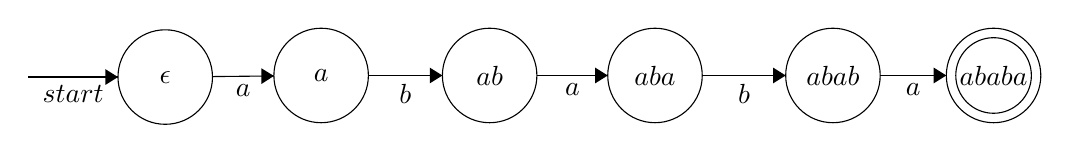
\begin{tikzpicture}[scale=0.2]
\tikzstyle{every node}+=[inner sep=0pt]
\draw [black] (15.1,-19.8) circle (3);
\draw (15.1,-19.8) node {$\epsilon$};

\draw [black] (25,-19.7) circle (3);
\draw (25,-19.7) node {$a$};
\draw [black] (35.7,-19.7) circle (3);
\draw (35.7,-19.7) node {$ab$};
\draw [black] (46.2,-19.7) circle (3);
\draw (46.2,-19.7) node {$aba$};
\draw [black] (57.5,-19.7) circle (3);
\draw (57.5,-19.7) node {$abab$};
\draw [black] (67.7,-19.7) circle (3);
\draw (67.7,-19.7) node {$ababa$};
\draw [black] (67.7,-19.7) circle (2.4);
\draw [black] (6.4,-19.8) -- (12.1,-19.8);
\fill [black] (12.1,-19.8) -- (11.3,-19.3) -- (11.3,-20.3);
\draw (9.25,-20.3) node [below] {$start$};
\draw [black] (18.1,-19.77) -- (22,-19.73);
\fill [black] (22,-19.73) -- (21.2,-19.24) -- (21.21,-20.24);
\draw (20.05,-20.26) node [below] {$a$};
\draw [black] (28,-19.7) -- (32.7,-19.7);
\fill [black] (32.7,-19.7) -- (31.9,-19.2) -- (31.9,-20.2);
\draw (30.35,-20.2) node [below] {$b$};
\draw [black] (38.7,-19.7) -- (43.2,-19.7);
\fill [black] (43.2,-19.7) -- (42.4,-19.2) -- (42.4,-20.2);
\draw (40.95,-20.2) node [below] {$a$};
\draw [black] (49.2,-19.7) -- (54.5,-19.7);
\fill [black] (54.5,-19.7) -- (53.7,-19.2) -- (53.7,-20.2);
\draw (51.85,-20.2) node [below] {$b$};
\draw [black] (60.5,-19.7) -- (64.7,-19.7);
\fill [black] (64.7,-19.7) -- (63.9,-19.2) -- (63.9,-20.2);
\draw (62.6,-20.2) node [below] {$a$};
\end{tikzpicture}
\end{center}

Но что делать, если в слове попадается буква, которая не ведет в следующий префикс? Будем проводить переходы в самы длинный префикс нашего состояния. То есть из состояния $aba$ по $b$ мы перейдем в состояние $ab$, которое является самым длинным его префиксом.

\begin{center}
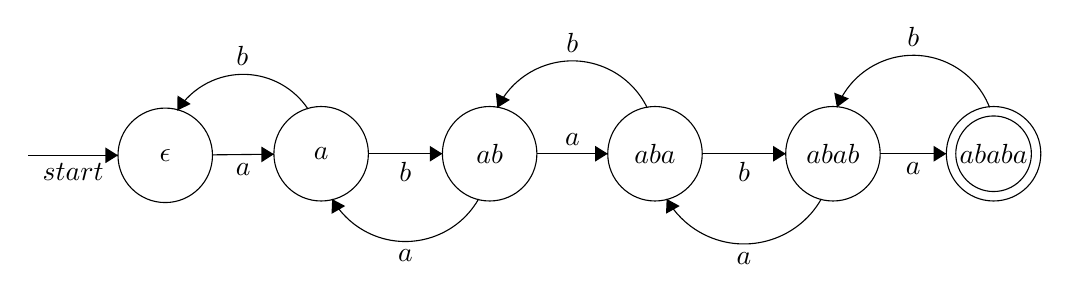
\begin{tikzpicture}[scale=0.2]
\tikzstyle{every node}+=[inner sep=0pt]
\draw [black] (15.1,-19.8) circle (3);
\draw (15.1,-19.8) node {$\epsilon$};

\draw [black] (25,-19.7) circle (3);
\draw (25,-19.7) node {$a$};
\draw [black] (35.7,-19.7) circle (3);
\draw (35.7,-19.7) node {$ab$};
\draw [black] (46.2,-19.7) circle (3);
\draw (46.2,-19.7) node {$aba$};
\draw [black] (57.5,-19.7) circle (3);
\draw (57.5,-19.7) node {$abab$};
\draw [black] (67.7,-19.7) circle (3);
\draw (67.7,-19.7) node {$ababa$};
\draw [black] (67.7,-19.7) circle (2.4);
\draw [black] (6.4,-19.8) -- (12.1,-19.8);
\fill [black] (12.1,-19.8) -- (11.3,-19.3) -- (11.3,-20.3);
\draw (9.25,-20.3) node [below] {$start$};
\draw [black] (18.1,-19.77) -- (22,-19.73);
\fill [black] (22,-19.73) -- (21.2,-19.24) -- (21.21,-20.24);
\draw (20.05,-20.26) node [below] {$a$};
\draw [black] (28,-19.7) -- (32.7,-19.7);
\fill [black] (32.7,-19.7) -- (31.9,-19.2) -- (31.9,-20.2);
\draw (30.35,-20.2) node [below] {$b$};
\draw [black] (38.7,-19.7) -- (43.2,-19.7);
\fill [black] (43.2,-19.7) -- (42.4,-19.2) -- (42.4,-20.2);
\draw (40.95,-19.2) node [above] {$a$};
\draw [black] (49.2,-19.7) -- (54.5,-19.7);
\fill [black] (54.5,-19.7) -- (53.7,-19.2) -- (53.7,-20.2);
\draw (51.85,-20.2) node [below] {$b$};
\draw [black] (60.5,-19.7) -- (64.7,-19.7);
\fill [black] (64.7,-19.7) -- (63.9,-19.2) -- (63.9,-20.2);
\draw (62.6,-20.2) node [below] {$a$};
\draw [black] (15.872,-16.948) arc (-212.49492:-326.34763:4.952);
\fill [black] (15.87,-16.95) -- (16.72,-16.54) -- (15.88,-16);
\draw (20,-14.15) node [above] {$b$};
\draw [black] (34.998,-22.577) arc (-29.76279:-150.23721:5.354);
\fill [black] (25.7,-22.58) -- (25.66,-23.52) -- (26.53,-23.02);
\draw (30.35,-25.77) node [below] {$a$};
\draw [black] (36.194,-16.782) arc (-205.86545:-334.13455:5.286);
\fill [black] (36.19,-16.78) -- (36.99,-16.28) -- (36.09,-15.84);
\draw (40.95,-13.3) node [above] {$b$};
\draw [black] (56.762,-22.571) arc (-29.63218:-150.36782:5.651);
\fill [black] (46.94,-22.57) -- (46.9,-23.51) -- (47.77,-23.02);
\draw (51.85,-25.93) node [below] {$a$};
\draw [black] (57.754,-16.752) arc (-201.43426:-338.56574:5.206);
\fill [black] (57.75,-16.75) -- (58.51,-16.19) -- (57.58,-15.82);
\draw (62.6,-12.95) node [above] {$b$};

\end{tikzpicture}
  \label{fig:AutKMP}
\end{center} 
Так мы продолжаем поиск с "нужного" нам момента. В итоге мы получим автомат с порядком $n$ состояний и прогнать по нему наш текст будет стоить нам $O(|t|)$. Дальше вопрос только в том, а сколько будет стоить нам построение данного автомата. Если искать суффиксы состояний полным перебором, то у нас будет $O(|w|^2)$.

\subsection{Алгоритм Кнута-Морриса-Пратта}
Построенный нами автомат называется ДКА Кнута-Морриса-Пратта (\ref{fig:AutKMP}). Определим новое понятие, которое поможет быстрее вычислить нужные на суффиксы.
\begin{Def}
\textit{Префикс - функция} $l: \Sigma^+ \rightarrow \Sigma^*$ функция, возвращающая самый длинный суффикс $y$ у непустого слова $x$, совпадающий с некоторым префиксом $x$, отличным от $x$.
\end{Def}

\begin{question}
Вычислите значение префикс-функции $l(w)$ для \textbf{a)} $a^n, n > 0$
\end{question}